\chapter{Power supply system design}
\section{System overview} \label{sec:literature_system}
A power regulation system for an AC power meter, compatible with both \SI{24}{VAC}/\SI{18}{VAC} inputs and capable of supplying 200mA, was designed and can be seen in  Fig.\ \ref{fig:system_diagram}. The high voltage \SI{240}{VAC} input to the transformer was stepped down to \SI{24}{VAC}/\SI{18}{VAC}, with a \SI{500}{\milli A} fuse for overcurrent protection. This output voltage was rectified to be used by the intermediary \SI{12}{VDC} stage, which fed into the final regulators for the \SI{+5}{VDC} and \SI{-5}{VDC} rail voltages, which was implemented using a linear regulator and a charge pump respectively.

\begin{figure}
    \centering
    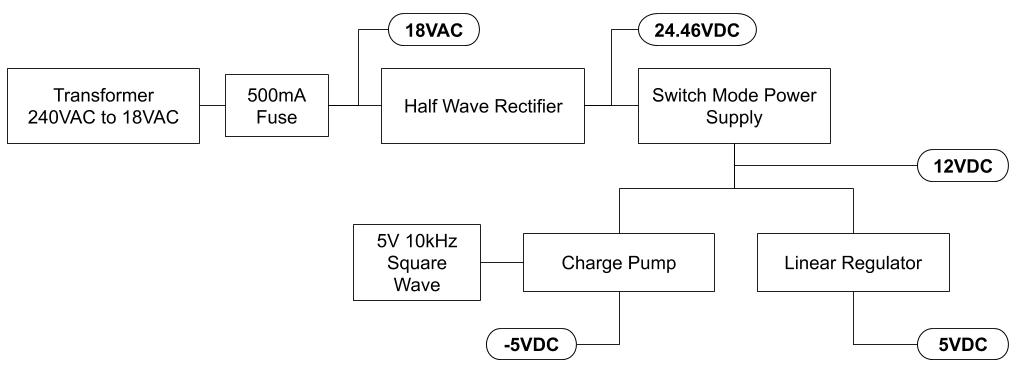
\includegraphics[width = 0.7\linewidth]{Figures/power_diagram.jpg}
    \caption{System diagram}
    \label{fig:system_diagram}
\end{figure}

\section{Rationale}\label{sec:rationale_system}
In order to supply the voltages for the \SI{5}{VDC} and \SI{-5}{VDC} power supplies the input had to be stepped down to \SI{12}{VDC} to minimize power losses in the linear regulator, protect the biasing transistor for the change pump, and not to exceed any maximum voltages if a \SI{24}{VAC} input was used.






